\chapter{Over netwerk applicaties}
Tegenwoordig heeft bijna elke applicatie wel ergens een netwerk nodig. Bij online games is dat evident, maar ook andere toepassingen houden steeds meer info bij in \textit{'the cloud'}. \textit{(Die cloud is niets meer dan een fancy woord om aan te duiden dat je informatie op een server opslaat.)} Ook wordt een online component dikwijls gebruikt om een licentie te controleren.

Toch is een netwerk applicatie een pak moeilijker te ontwikkelen dan een gewone, stand-alone applicatie. Enkele redenen daarvoor:

\begin{itemize}
\tick Je schrijf niet \'e\'en, maar twee programma's. Er moet namelijk ook een server geschreven worden.
\tick Data die je verstuurt over het netwerk bestaat enkel uit bits. Zowel de client als de server moeten die op dezelfde manier interpreteren.
\tick Een netwerk kan traag en onbetrouwbaar zijn. Je software moet dat zo goed mogelijk opvangen.
\tick Mobile apps hebben dikwijls weinig bandbreedte. Je mag niet meer data versturen dan strikt noodzakelijk is.
\end{itemize}

Het is dan ook erg belangrijk dat je het overzicht bewaart bij het onwikkelen van een netwerk applicatie. In de volgende hoofdstukken zullen we de delen van zo'n programma bestuderen. Hierin staan verschillende technieken beschreven die je helpen dat overzicht te bewaren. In ieder geval is het belangrijk om je project goed te structureren. In figuur \ref{fig:filetree} zie je een file tree van het voorbeeldproject.

\begin{figure}[ht]
\centering
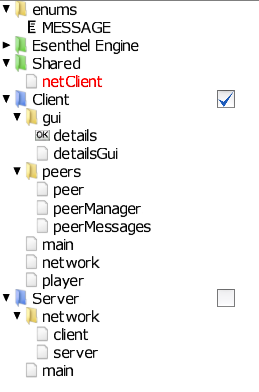
\includegraphics[width=0.3\linewidth]{../images/filetree.png}
\caption[]{Structuur van een client-server project.}
\label{fig:filetree}
\end{figure}

Je ziet dat zelfs een eenvoudig project al snel uit heel wat files bestaat. Je zet die niet allemaal in dezelfde map. Evident is dat we twee applicaties hebben: client en server. Maar het is zeker niet overbodig om ook binnen die applicaties folders te maken voor code die samen hoort. Zo heeft de client een folder voor alle gui elementen \textit{(zowel layout als code)} en een folder voor code i.v.m. peers \textit{(dat zijn andere spelers op het netwerk)}. We plaatsen dus ook de editor componenten niet zomaar in de root van het project. Immers, de server heeft dat gui element `details' helemaal niet nodig. Bij een verdere uitwerking zal de server waarschijnlijk zijn eigen gui elementen nodig hebben, waar de client dan weer niets aan heeft.

Daarnaast zie je ook een folder `enums'. Deze folder is w\'el beschikbaar voor elke app. We gebruiken enumeraties om berichten door te geven tussen de client en de server. Door ze in de root van het project te plaatsen zijn we zeker dat beide applicaties dezelfde lijst gebruiken.

Ook is er een library (groene folder) met de naam `Shared'. In deze folder plaatsen we alle code die zowel bij de client als de server hoort.

\begin{exercise}
Maak een nieuw project aan. Daarin maak je alvast alle folders en bestanden zoals in de afbeelding hierboven.
\end{exercise}

\section{Messages}
Data verzenden over het netwerk doe je via \texttt{Files}. Denk hierbij niet aan grote bestanden zoals op een harde schijf: elk bericht dat je verstuurt over het netwerk is in feite in klein bestandje. 

Aangezien je bij een file dient te vermelden hoe je het wil noemen, voordat je er data in kan zetten, moet je bij een netwerkfile aangeven dat het enkel om het bestand in het geheugen gaat. En omdat de ontvanger van het bericht moet weten over wat voor bericht het gaat, stuur als eerste byte steeds een enum met het type bericht. Hieronder zie je een voorbeeld van een dergelijk bestand, ditmaal om de positie van een speler te verzenden.

\begin{code}
File f;
f.writeMem();
f.putByte(M_CLIENT_POS);
f.putFlt(pos.x);
f.putFlt(pos.y);
\end{code}

Alle netwerkfuncties in de client en de server zullen dus steeds naar de eerste byte van een bericht kijken om te bepalen welke functie het bericht verder zal afhandelen. Je maakt best een enumeratie die alle mogelijke berichten bevat. In een groot programma kan ook een tweede byte geschakeld worden om een verdere onderverdeling te maken.

\begin{exercise} 
Maak in je project een enum `MESSAGE' met de volgende waarden: 
\begin{itemize}
	\item M\_CLIENT\_FULL
	\item M\_CLIENT\_POS
	\item M\_HELLO
	\item M\_ADD\_CLIENT
	\item M\_REMOVE\_CLIENT
\end{itemize}
\end{exercise}


